% =====================================================================
%  Aprendizaje No Supervisado — Unidad 2: Reducción de dimensionalidad
%  Sesiones 7 a 10 de la planeación didáctica
%  Compilar con: latexmk -pdf Unidad2-Reduccion_Dimensionalidad.tex
%  Las figuras se regeneran con: python3 figuras/generar_figuras.py
% =====================================================================
\documentclass[aspectratio=169,11pt]{beamer}

% ---------- Idioma y codificación ----------
\usepackage[utf8]{inputenc}
\usepackage[T1]{fontenc}
\usepackage[spanish,es-noshorthands,es-nodecimaldot]{babel}

% ---------- Paquetes ----------
\usepackage{amsmath,amssymb,bm}
\usepackage{booktabs,array}
\usepackage{listings}
\usepackage{tikz}
\usetikzlibrary{positioning,arrows.meta,calc,decorations.pathreplacing}
\graphicspath{{figuras/}}

% ---------- Tema y colores (coinciden con la planeación) ----------
\usetheme{Madrid}
\usefonttheme{professionalfonts}
\definecolor{marino}{HTML}{1F3864}
\definecolor{azul}{HTML}{2E75B6}
\definecolor{naranja}{HTML}{E07B22}
\definecolor{verde}{HTML}{5B9A3C}
\definecolor{fondocod}{HTML}{F4F6F9}
\setbeamercolor{palette primary}{bg=marino,fg=white}
\setbeamercolor{palette secondary}{bg=azul,fg=white}
\setbeamercolor{palette tertiary}{bg=marino,fg=white}
\setbeamercolor{frametitle}{bg=marino,fg=white}
\setbeamercolor{title}{bg=marino,fg=white}
\setbeamercolor{structure}{fg=azul}
\setbeamercolor{block title}{bg=azul,fg=white}
\setbeamercolor{block body}{bg=azul!8}
\setbeamercolor{block title alerted}{bg=naranja,fg=white}
\setbeamercolor{block body alerted}{bg=naranja!10}
\setbeamercolor{block title example}{bg=verde,fg=white}
\setbeamercolor{block body example}{bg=verde!10}
\setbeamercolor{alerted text}{fg=naranja}
\setbeamertemplate{navigation symbols}{}
\setbeamertemplate{itemize items}[circle]
\setbeamertemplate{blocks}[rounded][shadow=false]

% Diapositiva de sección automática
\AtBeginSection[]{
  \begin{frame}
    \vfill
    \centering
    \begin{beamercolorbox}[sep=12pt,center,rounded=true]{title}
      \usebeamerfont{title}\insertsectionhead
    \end{beamercolorbox}
    \vfill
  \end{frame}
}

% ---------- Código ----------
\lstdefinestyle{py}{
  language=Python,
  basicstyle=\ttfamily\scriptsize,
  keywordstyle=\color{marino}\bfseries,
  commentstyle=\color{gray}\itshape,
  stringstyle=\color{naranja},
  backgroundcolor=\color{fondocod},
  frame=single, rulecolor=\color{azul!40},
  showstringspaces=false, columns=fullflexible,
  breaklines=true, xleftmargin=4pt, xrightmargin=4pt
}
\lstset{style=py}

% ---------- Notación ----------
\newcommand{\R}{\mathbb{R}}
\newcommand{\x}{\bm{x}}
\newcommand{\z}{\bm{z}}
\newcommand{\uu}{\bm{u}}
\newcommand{\X}{\mathbf{X}}
\newcommand{\Sm}{\mathbf{S}}
\newcommand{\W}{\mathbf{W}}
\newcommand{\E}{\mathbb{E}}

% ---------- Datos de la presentación ----------
\title[Unidad 2: Reducción de dimensionalidad]{Unidad 2: Reducción de dimensionalidad}
\subtitle{Aprendizaje No Supervisado}
\author[A. Espinosa Romero]{Arturo Espinosa Romero}
\institute[FMAT]{Maestría en Inteligencia Artificial \\ Facultad de Matemáticas}
\date{Sesiones 7--10}

% =====================================================================
\begin{document}

\begin{frame}
  \titlepage
\end{frame}

\begin{frame}{Mapa de la unidad}
  \begin{columns}[T]
    \column{0.55\textwidth}
    \begin{enumerate}
      \item[\textbf{S7}] Análisis de componentes principales (PCA)
      \item[\textbf{S8}] PCA en la práctica y PCA con kernel
      \item[\textbf{S9}] Aprendizaje de variedades: MDS, Isomap y t-SNE
      \item[\textbf{S10}] Modelos de variables latentes y autoencoders
    \end{enumerate}
    \column{0.42\textwidth}
    \begin{block}{Entregables}
      \begin{itemize}
        \item Laboratorios de S7, S8 y S9
        \item Miniproyecto 2 (S10), 35\,\% de la calificación
      \end{itemize}
    \end{block}
  \end{columns}
  \vspace{6pt}
  \begin{alertblock}{Objetivo de la unidad}
    Aplicar e interpretar técnicas de reducción de dimensionalidad lineales y no
    lineales, y elegir la adecuada según el propósito del análisis.
  \end{alertblock}
\end{frame}

% =====================================================================
\section{Repaso y motivación}
% =====================================================================

\begin{frame}{¿Por qué reducir la dimensionalidad?}
  Tenemos $n$ observaciones $\x_i \in \R^d$ con $d$ grande. Buscamos una
  representación $\z_i \in \R^k$ con $k \ll d$ que conserve lo importante.
  \vspace{6pt}
  \begin{columns}[T]
    \column{0.5\textwidth}
    \begin{block}{Usos}
      \begin{itemize}
        \item \textbf{Visualización} ($k = 2$ o $3$)
        \item \textbf{Compresión} y almacenamiento
        \item \textbf{Eliminación de ruido}
        \item \textbf{Preprocesamiento} para agrupamiento (Unidad 1), detección de anomalías (Unidad 3) o modelos supervisados
      \end{itemize}
    \end{block}
    \column{0.46\textwidth}
    \begin{block}{Ejemplos de datos con $d$ grande}
      \begin{itemize}
        \item Imágenes: $28\times 28 = 784$ píxeles
        \item Expresión génica: $\sim 20\,000$ genes
        \item Texto: vocabularios de $10^4$--$10^5$ términos
        \item Sensores industriales: cientos de señales
      \end{itemize}
    \end{block}
  \end{columns}
\end{frame}

\begin{frame}{Repaso: la maldición de la dimensionalidad}
  \begin{columns}[c]
    \column{0.5\textwidth}
    \begin{itemize}
      \item El volumen crece como $r^d$: los datos se vuelven \alert{dispersos}.
      \item Las distancias se \alert{concentran}: el vecino más cercano y el más lejano están casi a la misma distancia.
      \item Métodos basados en distancias (k-medias, kNN, LOF) pierden poder discriminante.
      \item Se necesitan exponencialmente más datos para cubrir el espacio.
    \end{itemize}
    \vspace{4pt}
    {\small Experimento: 500 puntos uniformes en $[0,1]^d$ y un punto de consulta.}
    \column{0.48\textwidth}
    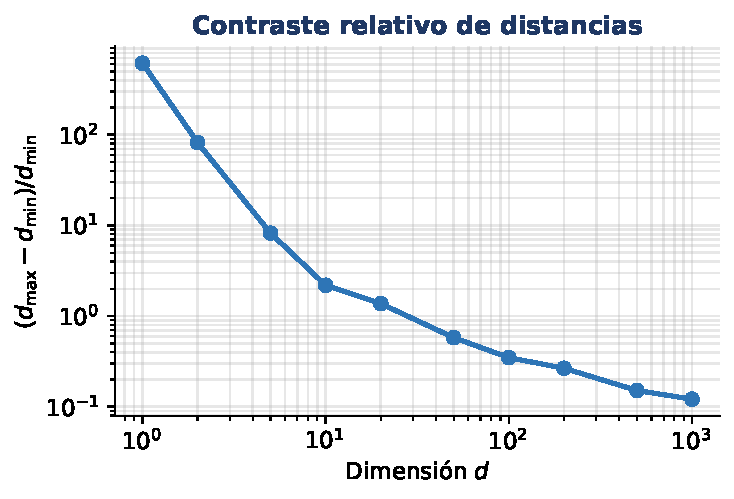
\includegraphics[width=\textwidth]{maldicion_dimensionalidad}
  \end{columns}
\end{frame}

\begin{frame}{La hipótesis de la variedad}
  \begin{columns}[c]
    \column{0.55\textwidth}
    Los datos reales de alta dimensión suelen vivir cerca de una
    \alert{variedad de baja dimensión} incrustada en $\R^d$.
    \vspace{6pt}
    \begin{itemize}
      \item Una imagen de un rostro tiene miles de píxeles, pero varía con pocos factores: pose, iluminación, expresión.
      \item La \textbf{dimensión intrínseca} es mucho menor que $d$.
      \item Reducir dimensionalidad = descubrir coordenadas para esa variedad.
    \end{itemize}
    \column{0.42\textwidth}
    \begin{block}{Dos familias}
      \textbf{Selección} de variables: conservar un subconjunto de las originales.\\[4pt]
      \textbf{Extracción} de variables: construir nuevas variables
      $\z = f(\x)$. \alert{Esta unidad.}
    \end{block}
  \end{columns}
\end{frame}

\begin{frame}{Panorama de métodos}
  \centering
  \renewcommand{\arraystretch}{1.25}
  \begin{tabular}{@{}llll@{}}
    \toprule
    \textbf{Método} & \textbf{Tipo} & \textbf{Preserva} & \textbf{Sesión}\\
    \midrule
    PCA                    & Lineal          & Varianza global               & S7--S8 \\
    PCA con kernel         & No lineal       & Varianza en espacio de rasgos & S8 \\
    MDS clásico            & Lineal          & Distancias euclidianas        & S9 \\
    Isomap                 & No lineal       & Distancias geodésicas         & S9 \\
    t-SNE                  & No lineal       & Vecindarios locales           & S9 \\
    PCA prob.\ / Análisis factorial & Lineal, prob.   & Covarianza                    & S10 \\
    ICA                    & Lineal          & Independencia estadística     & S10 \\
    Autoencoder            & No lineal       & Reconstrucción                & S10 \\
    \bottomrule
  \end{tabular}
\end{frame}

% =====================================================================
\section{Sesión 7: Análisis de componentes principales}
% =====================================================================

\begin{frame}{Idea geométrica}
  \centering
  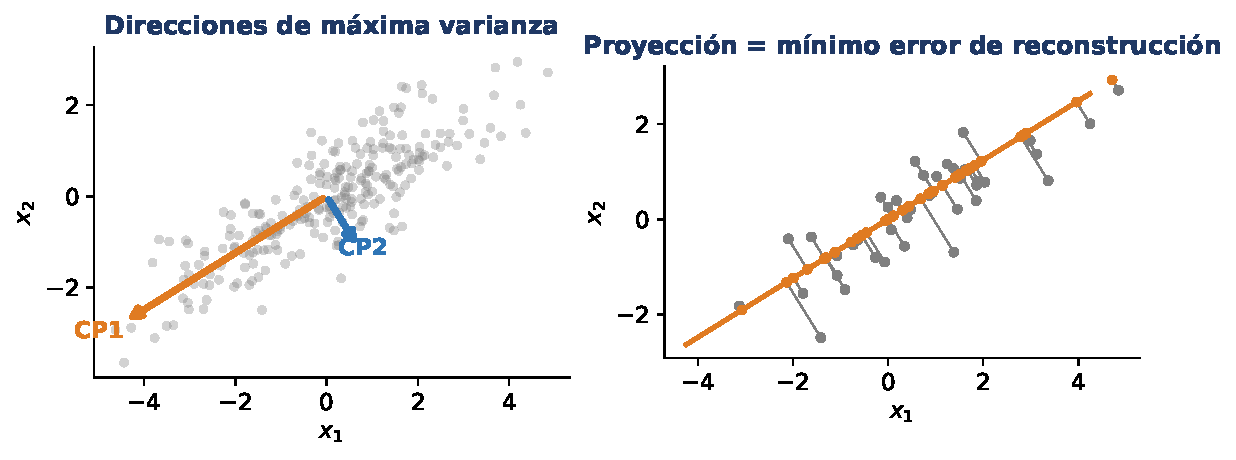
\includegraphics[width=0.85\textwidth]{pca_geometria}
  \vspace{2pt}
  \begin{itemize}
    \item Buscar las direcciones ortogonales en las que los datos \alert{varían más}.
    \item Equivalente: el subespacio cuya proyección \alert{pierde menos información}.
  \end{itemize}
\end{frame}

\begin{frame}{Planteamiento}
  Datos centrados $\x_1,\dots,\x_n \in \R^d$, con media
  $\bar{\x} = \frac{1}{n}\sum_i \x_i$ restada. Matriz de covarianza muestral:
  \[
    \Sm = \frac{1}{n-1}\sum_{i=1}^{n} (\x_i - \bar{\x})(\x_i - \bar{\x})^\top
        = \frac{1}{n-1}\X^\top\X .
  \]
  La proyección sobre una dirección unitaria $\uu$ es $z_i = \uu^\top \x_i$, con varianza
  \[
    \operatorname{Var}(z) = \frac{1}{n-1}\sum_i (\uu^\top\x_i)^2 = \uu^\top \Sm\, \uu .
  \]
  \begin{block}{Problema de optimización}
    \[
      \max_{\uu}\; \uu^\top \Sm\, \uu \qquad \text{sujeto a} \qquad \uu^\top\uu = 1 .
    \]
  \end{block}
\end{frame}

\begin{frame}{Solución: eigenvectores de la covarianza}
  Lagrangiano:
  $\mathcal{L}(\uu,\lambda) = \uu^\top \Sm\,\uu - \lambda(\uu^\top\uu - 1)$.
  \[
    \frac{\partial \mathcal{L}}{\partial \uu} = 2\Sm\,\uu - 2\lambda\uu = 0
    \quad\Longrightarrow\quad \Sm\,\uu = \lambda\,\uu .
  \]
  \begin{itemize}
    \item $\uu$ es un \alert{eigenvector} de $\Sm$ y la varianza proyectada es
          $\uu^\top\Sm\,\uu = \lambda$.
    \item La primera componente principal es el eigenvector del \textbf{mayor} eigenvalor $\lambda_1$.
    \item Las siguientes se obtienen imponiendo ortogonalidad: eigenvectores de
          $\lambda_2 \ge \lambda_3 \ge \dots \ge \lambda_d \ge 0$.
  \end{itemize}
  \begin{block}{Resultado}
    $\Sm = \mathbf{U}\boldsymbol{\Lambda}\mathbf{U}^\top$. Con
    $\mathbf{U}_k = [\uu_1,\dots,\uu_k]$, la representación reducida es
    $\z_i = \mathbf{U}_k^\top(\x_i - \bar{\x}) \in \R^k$.
  \end{block}
\end{frame}

\begin{frame}{Segunda visión: mínimo error de reconstrucción}
  Reconstrucción a partir de $k$ componentes:
  $\hat{\x}_i = \bar{\x} + \mathbf{U}_k\z_i = \bar{\x} + \mathbf{U}_k\mathbf{U}_k^\top(\x_i-\bar{\x})$.
  \[
    J_k = \frac{1}{n-1}\sum_{i=1}^n \lVert \x_i - \hat{\x}_i \rVert^2
        = \sum_{j=k+1}^{d} \lambda_j .
  \]
  \begin{itemize}
    \item Minimizar el error de reconstrucción $\Leftrightarrow$ maximizar la varianza retenida.
    \item El error es la suma de los eigenvalores \alert{descartados}.
    \item Proporción de varianza explicada por $k$ componentes:
          \[
            \rho_k = \frac{\sum_{j=1}^{k}\lambda_j}{\sum_{j=1}^{d}\lambda_j}.
          \]
  \end{itemize}
\end{frame}

\begin{frame}{PCA mediante la descomposición en valores singulares}
  Para $\X \in \R^{n\times d}$ centrada:
  \[
    \X = \mathbf{U}\boldsymbol{\Sigma}\mathbf{V}^\top
    \quad\Longrightarrow\quad
    \Sm = \frac{1}{n-1}\X^\top\X = \mathbf{V}\,\frac{\boldsymbol{\Sigma}^2}{n-1}\,\mathbf{V}^\top .
  \]
  \begin{itemize}
    \item Direcciones principales: columnas de $\mathbf{V}$.
    \item Eigenvalores: $\lambda_j = \sigma_j^2/(n-1)$.
    \item Puntuaciones (\emph{scores}): $\mathbf{Z} = \X\mathbf{V}_k = \mathbf{U}_k\boldsymbol{\Sigma}_k$.
  \end{itemize}
  \begin{alertblock}{¿Por qué SVD?}
    Es numéricamente más estable que formar $\X^\top\X$ (no eleva al cuadrado el número
    de condición) y es lo que usa \texttt{sklearn.decomposition.PCA}.
  \end{alertblock}
\end{frame}

\begin{frame}{Algoritmo}
  \begin{enumerate}
    \item Centrar los datos: $\X \leftarrow \X - \mathbf{1}\bar{\x}^\top$.
    \item (Opcional, pero usualmente necesario) \textbf{estandarizar} cada variable.
    \item Calcular la SVD: $\X = \mathbf{U}\boldsymbol{\Sigma}\mathbf{V}^\top$.
    \item Elegir $k$ (siguiente sesión).
    \item Proyectar: $\mathbf{Z} = \X\mathbf{V}_k$.
    \item Reconstruir, si se necesita: $\hat{\X} = \mathbf{Z}\mathbf{V}_k^\top + \mathbf{1}\bar{\x}^\top$.
  \end{enumerate}
  \vspace{6pt}
  \begin{alertblock}{¿Estandarizar o no?}
    PCA depende de la escala. Si una variable se mide en pesos y otra en miles de pesos,
    la primera dominará la varianza. Con unidades heterogéneas, estandarizar
    (equivale a hacer PCA sobre la matriz de \textbf{correlación}).
  \end{alertblock}
\end{frame}

\begin{frame}[fragile]{Laboratorio S7: PCA desde cero con NumPy}
\begin{lstlisting}
import numpy as np

def pca(X, k):
    mu = X.mean(axis=0)
    Xc = X - mu                                   # 1. centrar
    U, s, Vt = np.linalg.svd(Xc, full_matrices=False)  # 2. SVD
    componentes = Vt[:k]                          # direcciones principales (k x d)
    varianzas = s**2 / (len(X) - 1)               # eigenvalores
    Z = Xc @ componentes.T                        # 3. proyectar (n x k)
    return Z, componentes, varianzas, mu

def reconstruir(Z, componentes, mu):
    return Z @ componentes + mu

# Verificacion contra scikit-learn
from sklearn.decomposition import PCA
from sklearn.datasets import load_digits
X = load_digits().data
Z, C, var, mu = pca(X, 2)
Z_sk = PCA(2).fit_transform(X)
print(np.allclose(np.abs(Z), np.abs(Z_sk)))   # True: iguales salvo el signo
\end{lstlisting}
\end{frame}

\begin{frame}{Ejercicio guiado}
  \begin{exampleblock}{Calcula a mano}
    Sea $\Sm = \begin{pmatrix} 3 & 1\\ 1 & 3\end{pmatrix}$.
    \begin{enumerate}
      \item Encuentra sus eigenvalores y eigenvectores.
      \item ¿Qué proporción de la varianza explica la primera componente?
      \item ¿Cuál es el error de reconstrucción si se conserva sólo una componente?
    \end{enumerate}
  \end{exampleblock}
  \pause
  \begin{block}{Solución}
    $\lambda_1 = 4$ con $\uu_1 = \tfrac{1}{\sqrt{2}}(1,1)^\top$;
    $\lambda_2 = 2$ con $\uu_2 = \tfrac{1}{\sqrt{2}}(1,-1)^\top$.\\
    $\rho_1 = 4/6 \approx 67$\,\%. Error de reconstrucción: $J_1 = \lambda_2 = 2$.
  \end{block}
\end{frame}

% =====================================================================
\section{Sesión 8: PCA en la práctica y PCA con kernel}
% =====================================================================

\begin{frame}{¿Cuántas componentes conservar?}
  \begin{columns}[c]
    \column{0.55\textwidth}
    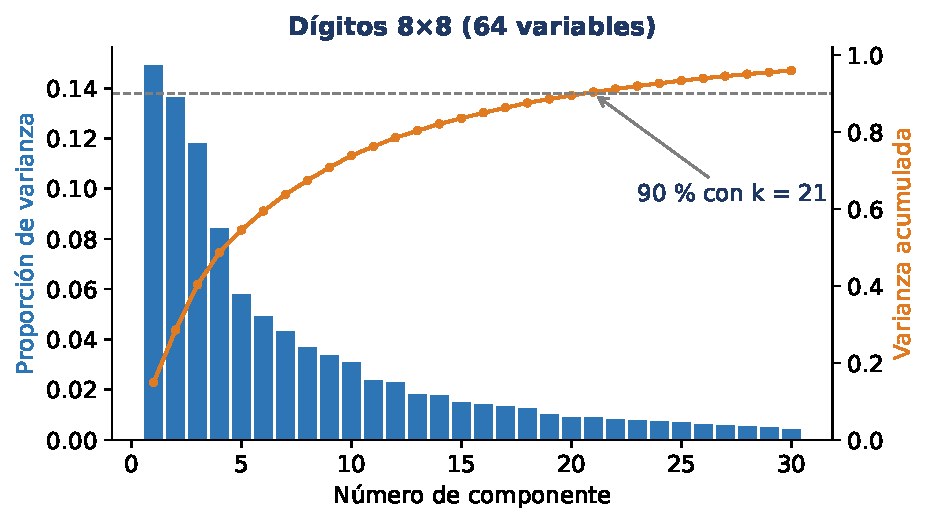
\includegraphics[width=\textwidth]{scree_digitos}
    \column{0.43\textwidth}
    \begin{itemize}
      \item \textbf{Umbral de varianza}: el menor $k$ con $\rho_k \ge 0.90$ (o 0.95).
      \item \textbf{Codo} en el gráfico de sedimentación (\emph{scree plot}).
      \item \textbf{Criterio de Kaiser}: $\lambda_j > 1$ (sólo con datos estandarizados).
      \item \textbf{Según la tarea}: validación cruzada del modelo que usa $\z$.
      \item Para visualizar: $k = 2$ o $3$.
    \end{itemize}
  \end{columns}
\end{frame}

\begin{frame}{Proyección de los dígitos en dos componentes}
  \begin{columns}[c]
    \column{0.5\textwidth}
    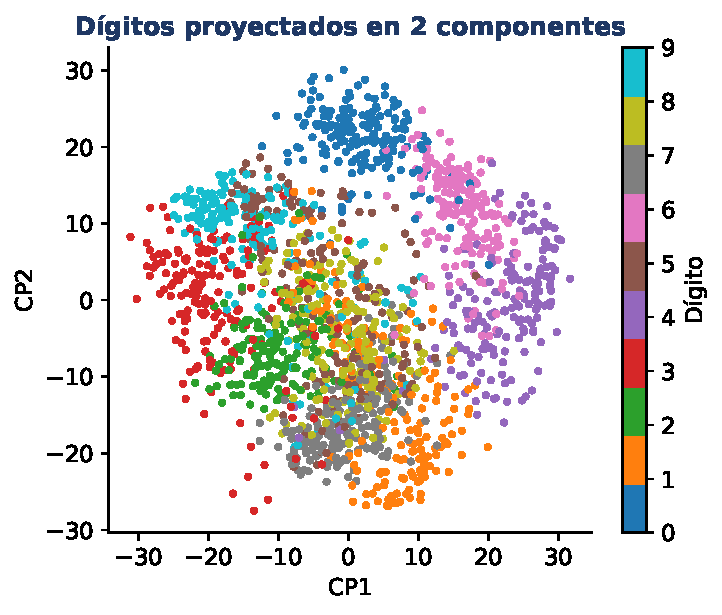
\includegraphics[width=\textwidth]{digitos_pca2}
    \column{0.48\textwidth}
    \begin{itemize}
      \item 1\,797 imágenes de $8\times8$ ($d = 64$).
      \item Dos componentes retienen $\approx 29$\,\% de la varianza.
      \item Algunos dígitos (0, 4, 6) se separan; otros se traslapan.
      \item PCA \alert{no usa las etiquetas}: el color sólo sirve para evaluar.
    \end{itemize}
    \vspace{4pt}
    \begin{alertblock}{Pregunta}
      ¿Qué dígitos se confunden y por qué?
    \end{alertblock}
  \end{columns}
\end{frame}

\begin{frame}{Reconstrucción y compresión}
  \begin{columns}[c]
    \column{0.45\textwidth}
    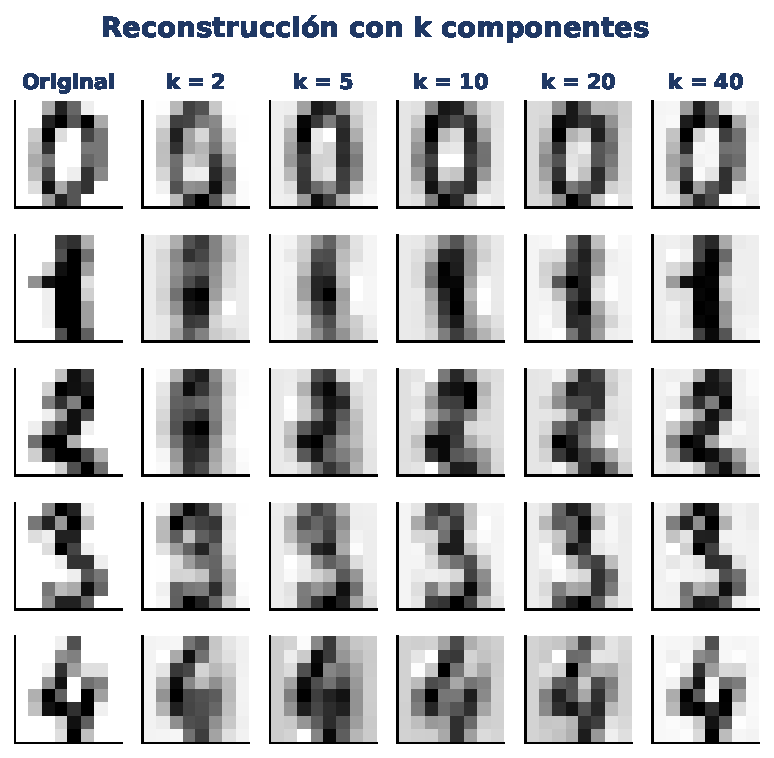
\includegraphics[width=\textwidth]{reconstruccion_digitos}
    \column{0.52\textwidth}
    \begin{itemize}
      \item Con $k = 10$ ya se reconoce el dígito; con $k = 20$ es casi idéntico.
      \item Factor de compresión: guardar $\z\in\R^{k}$ más $\mathbf{U}_k$ y $\bar{\x}$.
      \item Eliminación de ruido: el ruido se reparte en las componentes de menor varianza, que se descartan.
    \end{itemize}
  \end{columns}
\end{frame}

\begin{frame}{Interpretación: cargas y biplot}
  \begin{columns}[c]
    \column{0.52\textwidth}
    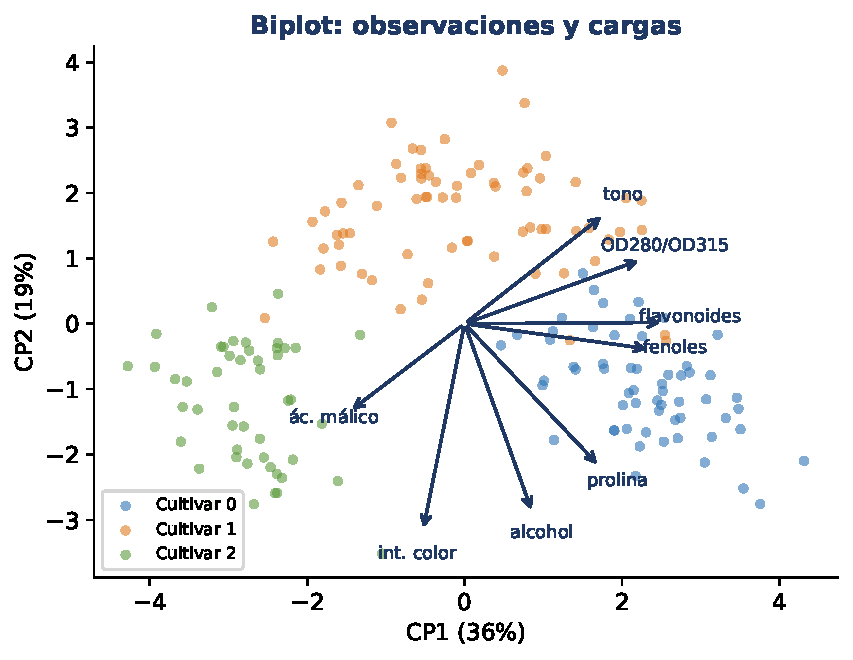
\includegraphics[width=\textwidth]{biplot_vinos}
    \column{0.46\textwidth}
    \begin{itemize}
      \item \textbf{Cargas} (\emph{loadings}): entradas de $\uu_j$; peso de cada variable original en la componente.
      \item Flechas en la misma dirección: variables \alert{correlacionadas}.
      \item Flechas opuestas: correlación negativa; perpendiculares: poca correlación.
      \item Puntos en la dirección de una flecha: valores altos de esa variable.
    \end{itemize}
    {\small Datos: 13 mediciones químicas de 178 vinos, estandarizadas.}
  \end{columns}
\end{frame}

\begin{frame}{Variantes para datos grandes}
  \renewcommand{\arraystretch}{1.3}
  \begin{tabular}{@{}>{\raggedright\arraybackslash}p{0.27\textwidth}>{\raggedright\arraybackslash}p{0.36\textwidth}>{\raggedright\arraybackslash}p{0.3\textwidth}@{}}
    \toprule
    \textbf{Variante} & \textbf{Idea} & \textbf{Cuándo usarla}\\
    \midrule
    PCA aleatorizado & Proyección aleatoria a un subespacio pequeño y SVD exacta en él &
      $n$ y $d$ grandes, $k$ pequeño \\
    PCA incremental & Actualiza la descomposición por lotes &
      Los datos no caben en memoria \\
    PCA disperso & Penalización $\ell_1$ sobre las cargas &
      Se requieren componentes interpretables \\
    TruncatedSVD & SVD sin centrar &
      Matrices dispersas (texto) \\
    \bottomrule
  \end{tabular}
  \vspace{6pt}
  {\small En scikit-learn: \texttt{PCA(svd\_solver="randomized")}, \texttt{IncrementalPCA},
  \texttt{SparsePCA}, \texttt{TruncatedSVD}.}
\end{frame}

\begin{frame}{Limitaciones de PCA}
  \begin{itemize}
    \item Sólo captura estructura \alert{lineal}.
    \item Máxima varianza no siempre significa máxima información útil.
    \item Sensible a valores atípicos (la varianza lo es).
    \item Sensible a la escala de las variables.
    \item Las componentes son combinaciones de todas las variables: pueden ser difíciles de interpretar.
  \end{itemize}
  \vspace{4pt}
  \centering
  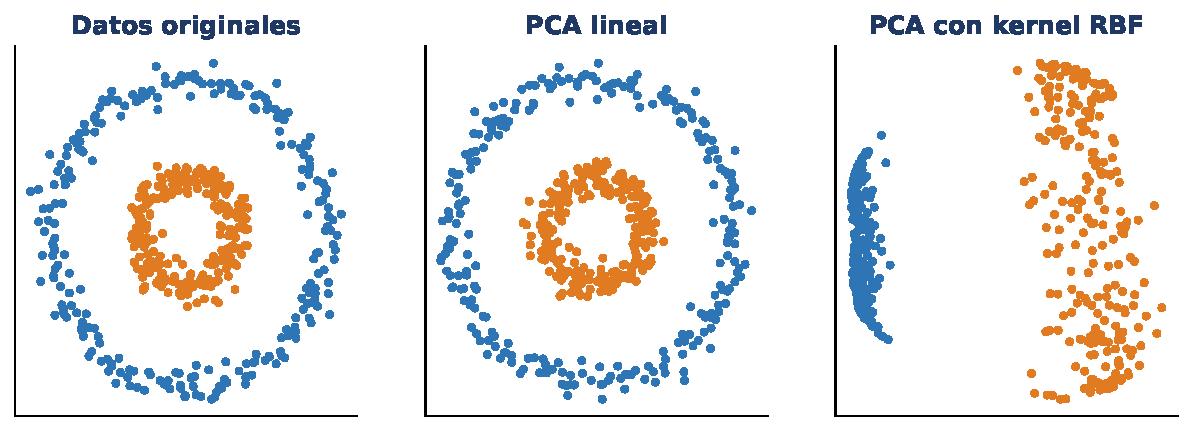
\includegraphics[width=0.75\textwidth]{kernel_pca_circulos}
\end{frame}

\begin{frame}{PCA con kernel: idea}
  Mapear los datos a un espacio de rasgos $\phi:\R^d\to\mathcal{H}$ y hacer PCA allí.
  \vspace{4pt}
  \begin{itemize}
    \item $\mathcal{H}$ puede tener dimensión enorme o infinita: no se calcula $\phi$ explícitamente.
    \item Sólo se necesitan productos internos:
          $k(\x_i,\x_j) = \langle\phi(\x_i),\phi(\x_j)\rangle$ (\alert{truco del kernel}).
  \end{itemize}
  \begin{block}{Kernels comunes}
    \begin{tabular}{@{}ll@{}}
      Lineal      & $k(\x,\x') = \x^\top\x'$ \quad (recupera PCA)\\
      Polinomial  & $k(\x,\x') = (\x^\top\x' + c)^p$ \\
      RBF (gaussiano) & $k(\x,\x') = \exp\!\left(-\gamma\lVert\x-\x'\rVert^2\right)$
    \end{tabular}
  \end{block}
\end{frame}

\begin{frame}{PCA con kernel: formulación}
  \begin{enumerate}
    \item Matriz kernel $\mathbf{K}_{ij} = k(\x_i,\x_j)$, de tamaño $n\times n$.
    \item Centrarla en el espacio de rasgos, con $\mathbf{1}_n$ la matriz de entradas $1/n$:
          \[
            \tilde{\mathbf{K}} = \mathbf{K} - \mathbf{1}_n\mathbf{K} - \mathbf{K}\mathbf{1}_n
                                + \mathbf{1}_n\mathbf{K}\mathbf{1}_n .
          \]
    \item Resolver $\tilde{\mathbf{K}}\bm{a}_j = n\lambda_j\bm{a}_j$ y normalizar
          $\bm{a}_j$ para que la componente en $\mathcal{H}$ tenga norma uno.
    \item Proyección de un punto: $z_j(\x) = \sum_{i=1}^{n} a_{ji}\,\tilde{k}(\x,\x_i)$.
  \end{enumerate}
  \begin{alertblock}{Costos y cuidados}
    Memoria $O(n^2)$ y tiempo $O(n^3)$. La reconstrucción (\emph{pre-imagen}) no es directa.
    Hiperparámetros como $\gamma$ se eligen con validación de la tarea final.
  \end{alertblock}
\end{frame}

\begin{frame}[fragile]{Laboratorio S8: PCA con scikit-learn}
\begin{lstlisting}
from sklearn.pipeline import make_pipeline
from sklearn.preprocessing import StandardScaler
from sklearn.decomposition import PCA, KernelPCA
from sklearn.datasets import load_digits, make_circles

X, y = load_digits(return_X_y=True)

# PCA conservando el 90% de la varianza
pca = make_pipeline(StandardScaler(), PCA(n_components=0.90))
Z = pca.fit_transform(X)
print(Z.shape, pca[-1].explained_variance_ratio_.sum())

# Cargas de la primera componente
cargas = pca[-1].components_[0]

# Reconstruccion
X_rec = pca.inverse_transform(Z)

# PCA con kernel sobre circulos concentricos
Xc, yc = make_circles(500, factor=0.35, noise=0.06, random_state=0)
Zk = KernelPCA(n_components=2, kernel="rbf", gamma=4).fit_transform(Xc)
\end{lstlisting}
\end{frame}

% =====================================================================
\section{Sesión 9: Aprendizaje de variedades}
% =====================================================================

\begin{frame}{Cuando la estructura no es lineal}
  \centering
  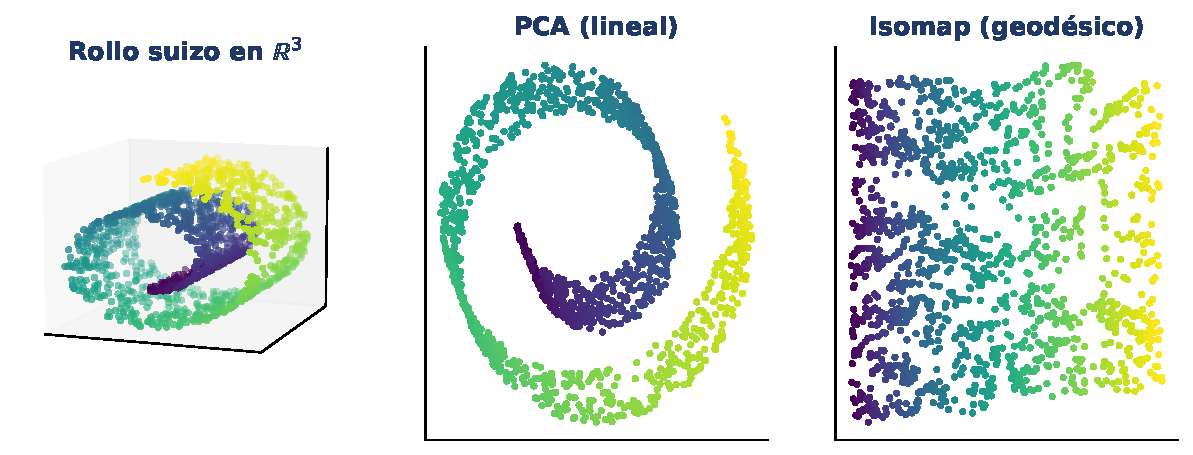
\includegraphics[width=0.95\textwidth]{rollo_suizo}
  \begin{itemize}
    \item El rollo suizo es una hoja 2D enrollada en $\R^3$.
    \item PCA \alert{aplasta} el rollo: puntos lejanos sobre la hoja quedan juntos.
    \item Isomap lo \alert{desenrolla}: respeta la distancia medida sobre la superficie.
  \end{itemize}
\end{frame}

\begin{frame}{Escalamiento multidimensional (MDS)}
  Dado sólo un conjunto de distancias $D_{ij}$, encontrar $\z_i\in\R^k$ con
  $\lVert\z_i - \z_j\rVert \approx D_{ij}$.
  \begin{block}{MDS clásico}
    \begin{enumerate}
      \item Doble centrado: $\mathbf{B} = -\tfrac{1}{2}\mathbf{J}\mathbf{D}^{(2)}\mathbf{J}$,
            con $\mathbf{J} = \mathbf{I} - \tfrac{1}{n}\mathbf{1}\mathbf{1}^\top$ y
            $\mathbf{D}^{(2)}_{ij} = D_{ij}^2$.
      \item Eigendescomposición $\mathbf{B} = \mathbf{V}\boldsymbol{\Lambda}\mathbf{V}^\top$.
      \item Coordenadas: $\mathbf{Z} = \mathbf{V}_k\boldsymbol{\Lambda}_k^{1/2}$.
    \end{enumerate}
  \end{block}
  \begin{itemize}
    \item Con distancias euclidianas, MDS clásico da el mismo resultado que PCA.
    \item \textbf{MDS métrico}: minimiza el \emph{stress}
          $\sum_{i<j}\bigl(D_{ij} - \lVert\z_i-\z_j\rVert\bigr)^2$ (algoritmo SMACOF).
    \item Útil cuando sólo se tienen disimilitudes (encuestas, distancias de edición).
  \end{itemize}
\end{frame}

\begin{frame}{Isomap: distancias geodésicas}
  \begin{columns}[c]
    \column{0.55\textwidth}
    \begin{enumerate}
      \item Construir el grafo de $k$ vecinos más cercanos, con aristas pesadas por la distancia euclidiana.
      \item Aproximar la distancia geodésica con la ruta más corta en el grafo (Dijkstra o Floyd-Warshall).
      \item Aplicar MDS clásico a la matriz de distancias geodésicas.
    \end{enumerate}
    \column{0.42\textwidth}
    \begin{alertblock}{Cuidados}
      \begin{itemize}
        \item $k$ pequeño: grafo desconectado.
        \item $k$ grande: ``atajos'' que cruzan la variedad.
        \item Sensible al ruido.
        \item Costo $O(n^2\log n)$ o más.
      \end{itemize}
    \end{alertblock}
  \end{columns}
  \vspace{8pt}
  \centering
  \begin{tikzpicture}[node distance=2.8cm, every node/.style={font=\small}]
    \node[draw=azul,fill=azul!10,rounded corners,minimum height=8mm] (a) {Datos $\x_i$};
    \node[draw=azul,fill=azul!10,rounded corners,minimum height=8mm,right=1.2cm of a] (b) {Grafo kNN};
    \node[draw=azul,fill=azul!10,rounded corners,minimum height=8mm,right=1.2cm of b] (c) {Rutas más cortas};
    \node[draw=naranja,fill=naranja!10,rounded corners,minimum height=8mm,right=1.2cm of c] (d) {MDS $\to\z_i$};
    \draw[-{Stealth},thick,marino] (a) -- (b);
    \draw[-{Stealth},thick,marino] (b) -- (c);
    \draw[-{Stealth},thick,marino] (c) -- (d);
  \end{tikzpicture}
\end{frame}

\begin{frame}{t-SNE: similitudes en alta dimensión}
  Convertir distancias en \alert{probabilidades de ser vecinos}.
  \[
    p_{j\mid i} = \frac{\exp\!\left(-\lVert\x_i-\x_j\rVert^2/2\sigma_i^2\right)}
                       {\sum_{l\neq i}\exp\!\left(-\lVert\x_i-\x_l\rVert^2/2\sigma_i^2\right)},
    \qquad
    p_{ij} = \frac{p_{j\mid i} + p_{i\mid j}}{2n}.
  \]
  \begin{itemize}
    \item Cada $\sigma_i$ se ajusta para que la distribución $P_i$ tenga una
          \textbf{perplejidad} fija:
          \[
            \operatorname{Perp}(P_i) = 2^{H(P_i)}, \qquad
            H(P_i) = -\sum_j p_{j\mid i}\log_2 p_{j\mid i}.
          \]
    \item La perplejidad es, informalmente, el \alert{número efectivo de vecinos} (típico: 5--50).
  \end{itemize}
\end{frame}

\begin{frame}{t-SNE: similitudes en baja dimensión y optimización}
  En el espacio de llegada se usa una \textbf{t de Student} con un grado de libertad:
  \[
    q_{ij} = \frac{\left(1+\lVert\z_i-\z_j\rVert^2\right)^{-1}}
                  {\sum_{l\neq m}\left(1+\lVert\z_l-\z_m\rVert^2\right)^{-1}} .
  \]
  Se minimiza la divergencia de Kullback-Leibler con descenso de gradiente:
  \[
    C = \mathrm{KL}(P\,\Vert\,Q) = \sum_{i\neq j} p_{ij}\log\frac{p_{ij}}{q_{ij}} .
  \]
  \begin{block}{¿Por qué colas pesadas?}
    Resuelve el \emph{problema de aglomeración}: en 2D no hay espacio para acomodar
    todas las distancias moderadas; la cola pesada permite alejar puntos disímiles.
  \end{block}
\end{frame}

\begin{frame}{Efecto de la perplejidad}
  \centering
  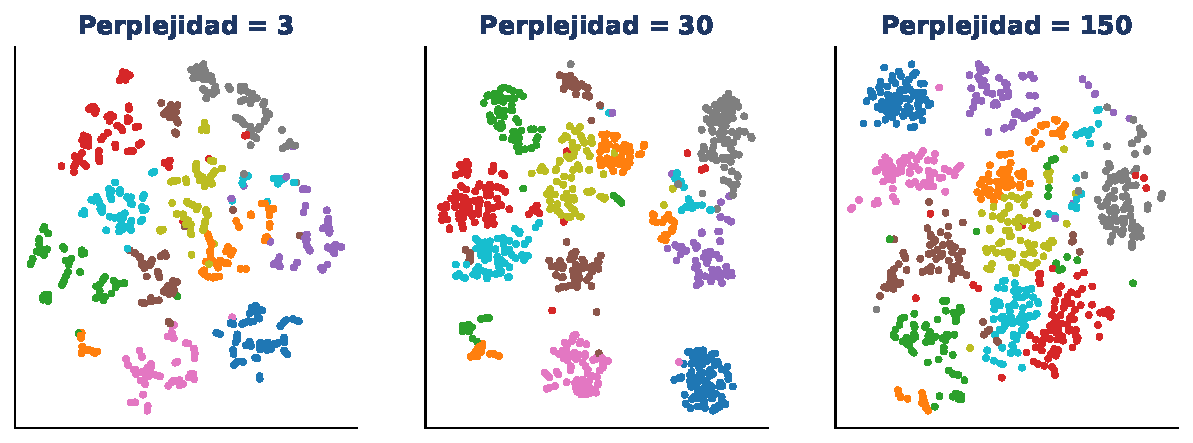
\includegraphics[width=0.92\textwidth]{tsne_perplejidad}
  \begin{itemize}
    \item Perplejidad baja: estructura muy local, grupos fragmentados.
    \item Perplejidad alta: más estructura global, grupos menos definidos.
    \item Siempre probar \alert{varios valores} y varias semillas.
  \end{itemize}
\end{frame}

\begin{frame}{Comparación en el conjunto de dígitos}
  \centering
  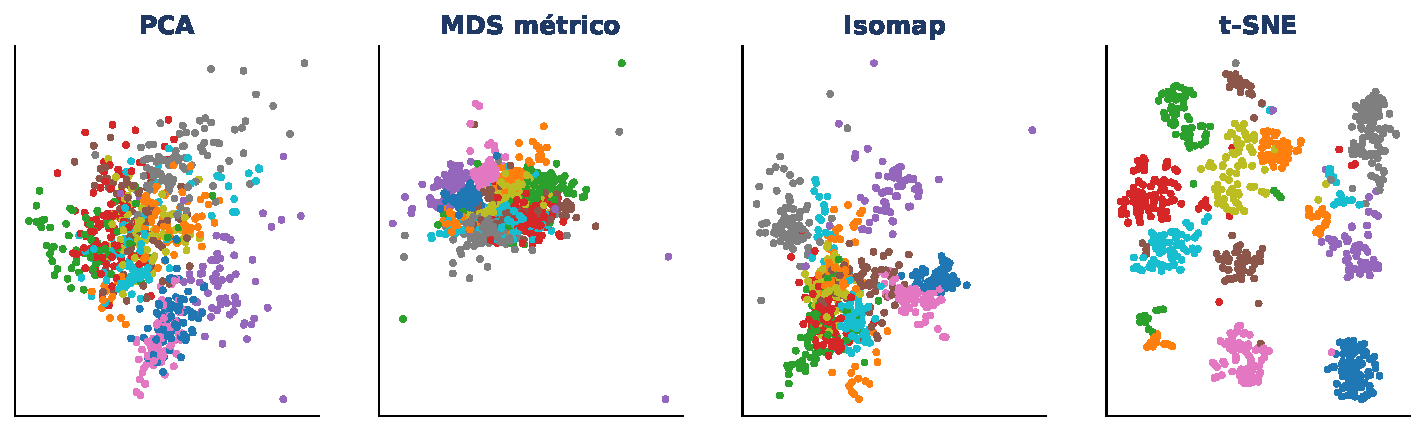
\includegraphics[width=\textwidth]{manifold_digitos}
  \vspace{2pt}
  \begin{itemize}
    \item 800 dígitos estandarizados, coloreados por su etiqueta (no usada por los métodos).
    \item Los métodos locales (t-SNE) separan mejor las clases que los globales (PCA, MDS).
    \item En el laboratorio se repite la comparación con Fashion-MNIST.
  \end{itemize}
\end{frame}

\begin{frame}{Cómo (no) leer un mapa t-SNE}
  \begin{alertblock}{Lo que \textbf{no} significa}
    \begin{itemize}
      \item El \textbf{tamaño} de un grupo no indica su dispersión real.
      \item La \textbf{distancia entre grupos} no es confiable.
      \item Los ejes no tienen interpretación.
      \item Ver grupos no prueba que existan: el ruido también puede formar grupos.
    \end{itemize}
  \end{alertblock}
  \begin{exampleblock}{Buenas prácticas}
    \begin{itemize}
      \item Reducir primero con PCA (p.\ ej.\ a 50 componentes) para acelerar y quitar ruido.
      \item Probar varios hiperparámetros y semillas; inicializar con PCA.
      \item Usarlos para \emph{explorar}, no como entrada directa de agrupamiento sin validar.
    \end{itemize}
  \end{exampleblock}
\end{frame}

\begin{frame}[fragile]{Laboratorio S9: comparación de proyecciones}
\begin{lstlisting}[basicstyle=\ttfamily\fontsize{6.5}{7.5}\selectfont]
import time
import numpy as np
from sklearn.datasets import fetch_openml
from sklearn.decomposition import PCA
from sklearn.manifold import MDS, Isomap, TSNE

# Fashion-MNIST: 70 000 imagenes de 28x28; usamos una muestra
X, y = fetch_openml("Fashion-MNIST", version=1, return_X_y=True, as_frame=False)
idx = np.random.default_rng(0).choice(len(X), 2000, replace=False)
X, y = X[idx] / 255.0, y[idx].astype(int)
X50 = PCA(50).fit_transform(X)                 # pre-reduccion recomendada
metodos = {
    "PCA":    PCA(2),
    "MDS":    MDS(2, random_state=0),
    "Isomap": Isomap(n_neighbors=10, n_components=2),
    "t-SNE":  TSNE(2, perplexity=30, init="pca", random_state=0),
}
proyecciones, tiempos = {}, {}
for nombre, m in metodos.items():
    t0 = time.perf_counter()
    proyecciones[nombre] = m.fit_transform(X50)
    tiempos[nombre] = time.perf_counter() - t0
# Graficar cada proyeccion coloreada por y; comparar tiempos
\end{lstlisting}
\end{frame}

% =====================================================================
\section{Sesión 10: Modelos de variables latentes y autoencoders}
% =====================================================================

\begin{frame}{Modelos generativos de variables latentes}
  Suponer que cada observación $\x\in\R^d$ se genera a partir de una variable oculta
  $\z\in\R^k$ con $k<d$:
  \[
    \z \sim p(\z), \qquad \x \mid \z \sim p(\x\mid\z).
  \]
  \begin{itemize}
    \item Da a PCA una interpretación \textbf{probabilística}.
    \item Permite verosimilitud, manejo de datos faltantes, selección de modelo y generación de datos nuevos.
    \item Base de la detección de anomalías por baja verosimilitud (Unidad 3).
  \end{itemize}
  \vspace{4pt}
  \centering
  \begin{tikzpicture}[every node/.style={font=\small}]
    \node[circle,draw=azul,fill=azul!10,minimum size=10mm] (z) {$\z$};
    \node[circle,draw=marino,fill=marino!15,minimum size=10mm,right=2.2cm of z] (x) {$\x$};
    \draw[-{Stealth},thick,marino] (z) -- node[above]{$\W\z+\bm{\mu}+\bm{\epsilon}$} (x);
    \node[below=1mm of z]{\scriptsize latente};
    \node[below=1mm of x]{\scriptsize observada};
  \end{tikzpicture}
\end{frame}

\begin{frame}{PCA probabilístico y análisis factorial}
  Modelo lineal gaussiano:
  \[
    \z\sim\mathcal{N}(\bm{0},\mathbf{I}_k), \qquad
    \x = \W\z + \bm{\mu} + \bm{\epsilon}, \qquad
    \x \sim \mathcal{N}\!\left(\bm{\mu},\; \W\W^\top + \bm{\Psi}\right).
  \]
  \begin{columns}[T]
    \column{0.48\textwidth}
    \begin{block}{PCA probabilístico (PPCA)}
      $\bm{\Psi} = \sigma^2\mathbf{I}$: ruido \textbf{isotrópico}.\\[3pt]
      La solución de máxima verosimilitud tiene $\W$ en el subespacio de las primeras
      $k$ componentes principales; $\sigma^2$ es el promedio de los eigenvalores descartados.
    \end{block}
    \column{0.48\textwidth}
    \begin{block}{Análisis factorial (FA)}
      $\bm{\Psi} = \operatorname{diag}(\psi_1,\dots,\psi_d)$: ruido distinto por variable.\\[3pt]
      Se ajusta con EM. Es invariante a la escala de cada variable.
      Muy usado en psicometría y ciencias sociales.
    \end{block}
  \end{columns}
  \vspace{4pt}
  {\small $\W$ sólo está identificada hasta una rotación: en FA se usan rotaciones (varimax)
  para mejorar la interpretación.}
\end{frame}

\begin{frame}{Análisis de componentes independientes (ICA)}
  \begin{columns}[c]
    \column{0.5\textwidth}
    \textbf{Problema de la fiesta de cóctel}: $m$ micrófonos registran mezclas de $m$ voces.
    \[
      \x = \mathbf{A}\bm{s}, \qquad \hat{\bm{s}} = \W\x, \quad \W\approx\mathbf{A}^{-1}.
    \]
    \begin{itemize}
      \item Supuesto: fuentes $s_j$ \alert{independientes} y \alert{no gaussianas} (a lo más una gaussiana).
      \item PCA sólo decorrelaciona; ICA busca independencia.
      \item Ambigüedades: escala, signo y orden de las fuentes.
    \end{itemize}
    \column{0.48\textwidth}
    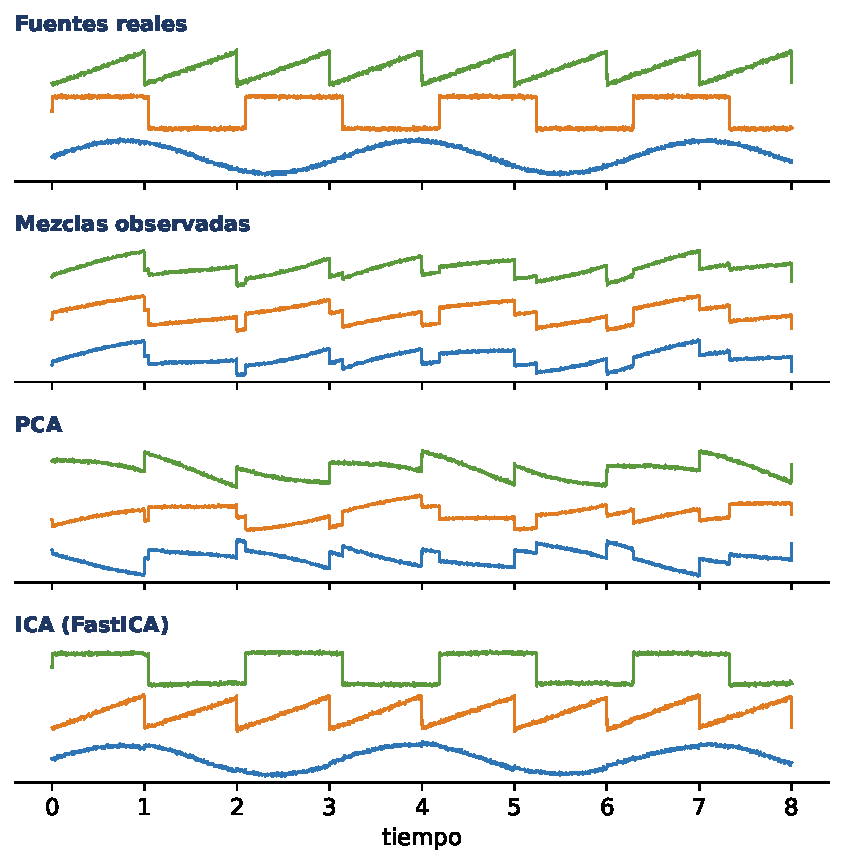
\includegraphics[width=\textwidth]{ica_coctel}
  \end{columns}
\end{frame}

\begin{frame}{ICA: cómo se estima}
  \textbf{Idea}: por el teorema central del límite, una mezcla es ``más gaussiana''
  que sus fuentes. Se busca $\W$ que haga $\hat{\bm{s}}$ lo \alert{menos gaussiana} posible.
  \begin{enumerate}
    \item Centrar y \textbf{blanquear} los datos (PCA con varianza unitaria).
    \item Maximizar una medida de no gaussianidad para cada componente:
      \begin{itemize}
        \item Curtosis: $\operatorname{kurt}(y) = \E[y^4] - 3\left(\E[y^2]\right)^2$.
        \item Negentropía: $J(y) = H(y_{\text{gauss}}) - H(y) \ge 0$, aproximada con funciones como $\log\cosh$.
      \end{itemize}
    \item Decorrelacionar las componentes estimadas (ortogonalización).
  \end{enumerate}
  \begin{exampleblock}{Aplicaciones}
    Separación de señales de audio, eliminación de artefactos en EEG/fMRI,
    señales financieras, extracción de rasgos en imágenes.
  \end{exampleblock}
\end{frame}

\begin{frame}{Autoencoders}
  \centering
  \begin{tikzpicture}[
      neu/.style={circle,draw=marino,fill=azul!15,minimum size=4.5mm,inner sep=0},
      lat/.style={circle,draw=naranja,fill=naranja!25,minimum size=4.5mm,inner sep=0},
      every node/.style={font=\small}]
    \foreach \i in {1,...,6} \node[neu] (a\i) at (0,{-0.55*\i}) {};
    \foreach \i in {1,...,4} \node[neu] (b\i) at (1.8,{-0.55*\i-0.55}) {};
    \foreach \i in {1,...,2} \node[lat] (c\i) at (3.6,{-0.55*\i-1.1}) {};
    \foreach \i in {1,...,4} \node[neu] (d\i) at (5.4,{-0.55*\i-0.55}) {};
    \foreach \i in {1,...,6} \node[neu] (e\i) at (7.2,{-0.55*\i}) {};
    \foreach \i in {1,...,6} \foreach \j in {1,...,4} \draw[gray!50] (a\i) -- (b\j);
    \foreach \i in {1,...,4} \foreach \j in {1,...,2} \draw[gray!50] (b\i) -- (c\j);
    \foreach \i in {1,...,2} \foreach \j in {1,...,4} \draw[gray!50] (c\i) -- (d\j);
    \foreach \i in {1,...,4} \foreach \j in {1,...,6} \draw[gray!50] (d\i) -- (e\j);
    \node at (0,-4.0) {$\x$};
    \node at (3.6,-4.0) {$\z = f_\theta(\x)$};
    \node at (7.2,-4.0) {$\hat{\x} = g_\phi(\z)$};
    \draw[decorate,decoration={brace,amplitude=5pt,mirror},thick,azul] (-0.2,-4.4) -- (3.4,-4.4)
      node[midway,below=5pt]{codificador};
    \draw[decorate,decoration={brace,amplitude=5pt,mirror},thick,azul] (3.8,-4.4) -- (7.4,-4.4)
      node[midway,below=5pt]{decodificador};
  \end{tikzpicture}
  \[
    \min_{\theta,\phi}\; \frac{1}{n}\sum_{i=1}^{n}\bigl\lVert \x_i - g_\phi\bigl(f_\theta(\x_i)\bigr)\bigr\rVert^2
  \]
\end{frame}

\begin{frame}{Autoencoders: propiedades y variantes}
  \begin{itemize}
    \item El \alert{cuello de botella} ($k<d$) obliga a aprender una representación compacta.
    \item Autoencoder \textbf{lineal} con pérdida cuadrática: aprende el mismo subespacio que PCA
          (Baldi y Hornik, 1989), aunque no necesariamente con base ortogonal.
    \item Con activaciones no lineales generaliza PCA a variedades curvas.
  \end{itemize}
  \vspace{4pt}
  \begin{tabular}{@{}ll@{}}
    \toprule
    \textbf{Variante} & \textbf{Idea}\\
    \midrule
    Con eliminación de ruido & Reconstruir $\x$ a partir de una versión corrupta $\tilde{\x}$\\
    Disperso & Penalizar la activación de $\z$\\
    Convolucional & Capas convolucionales para imágenes\\
    Variacional (VAE) & $\z$ con distribución; modelo generativo\\
    \bottomrule
  \end{tabular}
  \vspace{4pt}
  {\small El error de reconstrucción servirá como puntuación de anomalía en la Unidad 3.}
\end{frame}

\begin{frame}[fragile]{Laboratorio S10: autoencoder con PyTorch}
\begin{lstlisting}
import torch
from torch import nn

class Autoencoder(nn.Module):
    def __init__(self, d, k):
        super().__init__()
        self.codificador = nn.Sequential(nn.Linear(d, 32), nn.ReLU(), nn.Linear(32, k))
        self.decodificador = nn.Sequential(nn.Linear(k, 32), nn.ReLU(), nn.Linear(32, d))
    def forward(self, x):
        return self.decodificador(self.codificador(x))

X = torch.tensor(X_escalada, dtype=torch.float32)        # n x d
modelo = Autoencoder(d=X.shape[1], k=2)
opt = torch.optim.Adam(modelo.parameters(), lr=1e-3)
for epoca in range(200):
    opt.zero_grad()
    perdida = nn.functional.mse_loss(modelo(X), X)
    perdida.backward()
    opt.step()

Z = modelo.codificador(X).detach().numpy()              # representacion 2D
\end{lstlisting}
\end{frame}

\begin{frame}[fragile]{Laboratorio S10: FA e ICA con scikit-learn}
\begin{lstlisting}
from sklearn.decomposition import FactorAnalysis, FastICA, PCA

# Analisis factorial con rotacion varimax
fa = FactorAnalysis(n_components=3, rotation="varimax").fit(X_escalada)
cargas = fa.components_            # k x d
ruido = fa.noise_variance_         # diagonal de Psi

# Comparar log-verosimilitud promedio de PPCA y FA
print(PCA(3).fit(X_escalada).score(X_escalada),
      fa.score(X_escalada))

# ICA: separar fuentes a partir de mezclas
ica = FastICA(n_components=3, whiten="unit-variance", random_state=0)
S_est = ica.fit_transform(X_mezclas)   # fuentes estimadas
A_est = ica.mixing_                    # matriz de mezcla estimada
\end{lstlisting}
\end{frame}

% =====================================================================
\section{Cierre de la unidad}
% =====================================================================

\begin{frame}{¿Qué método elegir?}
  \centering
  \begin{tikzpicture}[
      q/.style={draw=marino,fill=azul!10,rounded corners,align=center,font=\small,minimum height=8mm},
      r/.style={draw=naranja,fill=naranja!12,rounded corners,align=center,font=\small,minimum height=7mm},
      lab/.style={font=\scriptsize,midway,fill=white,inner sep=1pt},
      >={Stealth}]
    \node[q] (q1) at (0,0) {¿Para qué se usará $\z$?};
    \node[q] (q2) at (-3.8,-1.7) {¿La estructura es lineal?};
    \node[q] (q4) at (3.8,-1.7) {¿Sólo se tienen disimilitudes?};
    \node[q] (q3) at (-5.4,-3.4) {¿Se buscan fuentes\\independientes?};
    \node[r] (r4) at (-1.6,-3.4) {PCA con kernel,\\Isomap, autoencoder};
    \node[r] (r3) at (-6.6,-5.1) {ICA};
    \node[r] (r2) at (-4.0,-5.1) {PCA (o PPCA / FA)};
    \node[r] (r5) at (2.4,-3.4) {MDS};
    \node[r] (r1) at (5.4,-3.4) {t-SNE};
    \draw[->,thick,marino] (q1) -- node[lab]{preprocesar / comprimir} (q2);
    \draw[->,thick,marino] (q1) -- node[lab]{visualizar / explorar} (q4);
    \draw[->,thick,marino] (q2) -- node[lab]{sí} (q3);
    \draw[->,thick,marino] (q2) -- node[lab]{no} (r4);
    \draw[->,thick,marino] (q3) -- node[lab]{sí} (r3);
    \draw[->,thick,marino] (q3) -- node[lab]{no} (r2);
    \draw[->,thick,marino] (q4) -- node[lab]{sí} (r5);
    \draw[->,thick,marino] (q4) -- node[lab]{no} (r1);
  \end{tikzpicture}
\end{frame}

\begin{frame}{Resumen}
  \renewcommand{\arraystretch}{1.2}
  \small
  \begin{tabular}{@{}lccccc@{}}
    \toprule
    & \textbf{Lineal} & \textbf{Proyecta nuevos} & \textbf{Reconstruye} & \textbf{Escala a $n$ grande} & \textbf{Interpretable}\\
    \midrule
    PCA            & sí & sí & sí & sí & media \\
    PCA con kernel & no & sí & difícil & no & baja \\
    MDS / Isomap   & --/no & no & no & no & baja \\
    t-SNE          & no & no & no & medio & baja \\
    PPCA / FA      & sí & sí & sí & sí & alta (FA) \\
    ICA            & sí & sí & sí & sí & alta \\
    Autoencoder    & no & sí & sí & sí & baja \\
    \bottomrule
  \end{tabular}
  \vspace{8pt}
  \begin{block}{Ideas clave}
    Estandarizar y centrar; elegir $k$ con un criterio explícito; validar contra la tarea final;
    no sobreinterpretar visualizaciones no lineales.
  \end{block}
\end{frame}

\begin{frame}{Miniproyecto 2: reducción de dimensionalidad}
  \begin{columns}[T]
    \column{0.55\textwidth}
    \begin{block}{Encargo}
      Elegir un conjunto de datos real con $d \ge 30$ variables de un sector productivo
      o social y:
      \begin{enumerate}
        \item Preparar y estandarizar los datos.
        \item Aplicar PCA, justificar $k$ e interpretar las cargas.
        \item Comparar con al menos dos métodos no lineales.
        \item Discutir qué decisiones informa la representación obtenida.
      \end{enumerate}
    \end{block}
    \column{0.41\textwidth}
    \begin{exampleblock}{Entrega (S10)}
      \begin{itemize}
        \item Notebook reproducible
        \item Informe breve con la interpretación
        \item Peso: 35\,\% de la calificación
      \end{itemize}
    \end{exampleblock}
    \begin{alertblock}{Pregunta guía}
      ¿Cuándo puede una visualización t-SNE llevar a una decisión equivocada?
    \end{alertblock}
  \end{columns}
\end{frame}

\begin{frame}{Lecturas de la unidad}
  \begin{itemize}
    \item James, G., Witten, D., Hastie, T., Tibshirani, R. y Taylor, J. (2023).
          \emph{An Introduction to Statistical Learning with Applications in Python}.
          Springer. \alert{Cap.~12.2: Principal Components Analysis.}
    \item Bishop, C.\,M. (2006). \emph{Pattern Recognition and Machine Learning}.
          Springer. \alert{Cap.~12: Continuous Latent Variables} (PCA, PPCA, FA, kernel PCA, ICA).
    \item Murphy, K.\,P. (2022). \emph{Probabilistic Machine Learning: An Introduction}.
          MIT Press. \alert{Cap.~20: Dimensionality Reduction} (PCA, FA, autoencoders, manifold learning).
    \item Hinton, G.\,E. y Sejnowski, T.\,J. (Eds.) (1999). \emph{Unsupervised Learning:
          Foundations of Neural Computation}. MIT Press. (Complementaria.)
  \end{itemize}
  \vspace{4pt}
  {\small Artículos originales: van der Maaten y Hinton (2008), t-SNE;
  Tenenbaum, de Silva y Langford (2000), Isomap.}
\end{frame}

\end{document}
